\documentclass{beamer}
\usepackage[italian]{babel}
\usepackage[latin1]{inputenc}
\usepackage{amsmath}
\usepackage{amssymb}
\usepackage{latexsym}
%\usepackage{pgfplots}
\usepackage{listings}
\usepackage{graphicx}
\usepackage{etoolbox}
\usepackage{subfiles}
\usepackage{verbatim}
\AfterEndEnvironment{lstlisting}{\leavevmode}
\usepackage{xcolor}
\usepackage{tikz}
\usetikzlibrary{quotes,angles,positioning}
\usepackage{xcolor} % for setting colors
% set the default code style
\lstset{
    language=Prolog,
    breaklines = true,
    basicstyle=\ttfamily\scriptsize,
    tabsize=3,
    showstringspaces=false,
    numbers=none,
    %keywordstyle=\color{blue},
    %stringstyle=\color{red},
    commentstyle=\color{gray}
}


\usetheme{Szeged}
%\usetheme{Darmstadt}
%\usetheme{Frankfurt}
%\usetheme{AnnArbor}
%\usetheme{Berkeley}
%\usetheme{Madrid}
%\usetheme{Hannover}
%\usetheme{Luebeck}
%\usetheme{Berlin}
%\usetheme{Rochester}
%\usetheme{default}
%\usetheme{Warsaw}

%\usecolortheme{spruce}
\usecolortheme{dolphin}
%\usecolortheme{rose}
%\usecolortheme{seahorse}
%\usecolortheme{whale}
%\setbeamertemplate{navigation symbols}{}

%------------------------------------------------------------
%This block of code defines the information to appear in the
%Title page
\titlegraphic{\hfill
\includegraphics[scale=0.05]{img/logo_unipr.png}}
\title {JSetL: a Java library to support Constraint Logic Programming}

\author[Vetere F.] {
\large{\textsc{Author}: Francesco Vetere\\ \small \textsc{e-mail:} \href{mailto:francesco.vetere@studenti.unipr.it}{francesco.vetere@studenti.unipr.it} }
}



\institute[University of Parma]
{
\textsc{University of Parma}
}

\date {\textsc{A.Y. 2019/2020}}

%End of title page configuration block
%------------------------------------------------------------

\usepackage{algorithm}
\usepackage{algpseudocode}
\renewcommand{\algorithmicrequire}{\textbf{Input:}}
\renewcommand{\algorithmicensure}{\textbf{Output:}}

\begin{document}

%The next statement creates the title page.
\begin{frame}
\maketitle
\end{frame}

%This block of code is for the table of contents after
%the title page
%\begin{frame}
%\frametitle{Sommario}
%\tableofcontents
%\end{frame}

\section{Logic Programming}
\begin{frame}{Logic Programming}
\begin{itemize}
\item \textbf{Declarative programming} is a programming style in which, generally speaking, the
programmer provides the properties that the desired solution should have, rather than specifying the actual sequence of operations needed in order to obtain that solution.
\item \textbf{Logic programming} is a declarative programming paradigm based on formal logic: basically, any program is composed by a list of \emph{facts} and \emph{rules}.\\
Given a certain \textit{goal}, the program tries to demonstrate the truth of the goal using the \emph{knowledge base} that the programmer provided.
\end{itemize}
\end{frame}

\begin{frame}{Unification}
A key concept in logic programming is the one of unification.\\
\begin{itemize}
\item In logic, \textbf{unification} is the algorithmic procedure used in solving equations involving symbolic expressions. \\
\item In other words, by replacing certain sub-expression variables with other expressions, unification tries to \textbf{identify two symbolic expressions}.\\
\item We say that two terms unify if they are the same term or if they contain variables that can be uniformly instantiated with terms in such a way that the resulting terms are equal. \\
\item In \textbf{Prolog}, for example, when we try to unify two terms, the interpreter performs all the necessary variable instantiations, so that the terms really are equal afterwards: if the unification succeeds, Prolog also gives us the value of the instantiated variables.
\end{itemize}
\end{frame}

\begin{frame}[fragile]
\frametitle{Logic programming in Prolog}
\begin{columns}
		\column{0.7\textwidth}
        	Let's see a basic example in Prolog:
		\column{0.3\textwidth}
			
\includegraphics[scale=0.15]{img/logo_swipl.png}
	\end{columns}


\begin{exampleblock}{family.pl}
    \lstinputlisting[basicstyle=\ttfamily\scriptsize]{code/family.pl}
\end{exampleblock}

Let's now query our program:\\

\begin{lstlisting}
?- grandfather(a, c).
true.
?- grandfather(X, c).
X = a .
\end{lstlisting}

\end{frame}

\section{Constraint Logic Programming}
\begin{frame}{Constraint Logic Programming}

\begin{itemize}
\setlength\itemsep{2em}
\item \textbf{Constraint Logic Programming} (\emph{CLP}) is a form of logic programming in which the user can explicitly manipulate \emph{constraints} (= relations over certain domains).\\
\item Basically, it's an extension of the logic paradigm, in which we allow the user to use constraints into rules.\\
These kind of problems are often called \textbf{Constraint Satisfaction Problems} (\emph{CSP}), and Prolog supports them through different modules, like \emph{clpfd}.
\end{itemize}

\end{frame}

\begin{frame}{SEND + MORE = MONEY}
\begin{columns}
		\column{0.5\textwidth}
        	\begin{itemize}
			\item Let's analyze a classic CSP, the SEND + MORE = MONEY puzzle.\\
			\item It is a cryptarithmetic problem, in which we want to find numeric values for the letters S,E,N,D,M,O,R,Y, such that, if they are considered in decimal ordering, the equation holds.
			\end{itemize}

		\column{0.5\textwidth}
			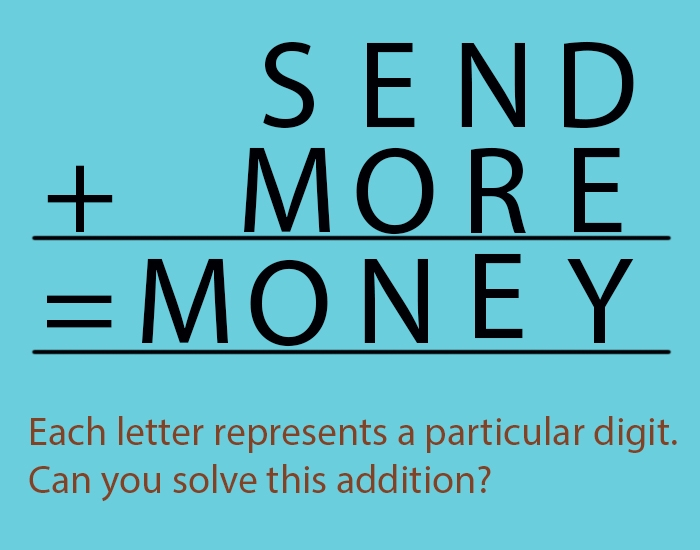
\includegraphics[scale=0.2]{img/money.jpg}
	\end{columns}
\end{frame}


\begin{frame}[fragile]
\frametitle{SEND + MORE = MONEY in Prolog}

Let's see the solution in Prolog:

\begin{exampleblock}{money.pl}
    \begin{lstlisting}[mathescape]
	:- use_module(library(clpfd)).

	money(S, E, N, D, M, O, R, Y) :-
		[S,E,N,D,M,O,R,Y] ins 0..9,
		all_different([S, E, N, D, M, O, R, Y]),
		S $\color{red} \#>=$ 1, M $\color{red} \#>=$ 1,
		1000*S + 100*E + 10*N + 1*D +
		1000*M + 100*O + 10*R + 1*E $\color{red} \#=$
		10000*M + 1000*O + 100*N + 10*E + 1*Y,
		label([S, E, N, D, M, O, R, Y]).
		
\end{lstlisting}
\end{exampleblock}
	\begin{columns}
		\column{0.7\textwidth}
Let's now query our program:
        	\begin{lstlisting}
			?- money(S, E, N, D, M, O, R, Y).
			S = 9, E = 5, N = 6, D = 7,
			M = 1, O = 0, R = 8, Y = 2.
			\end{lstlisting}
		\column{0.3\textwidth}
			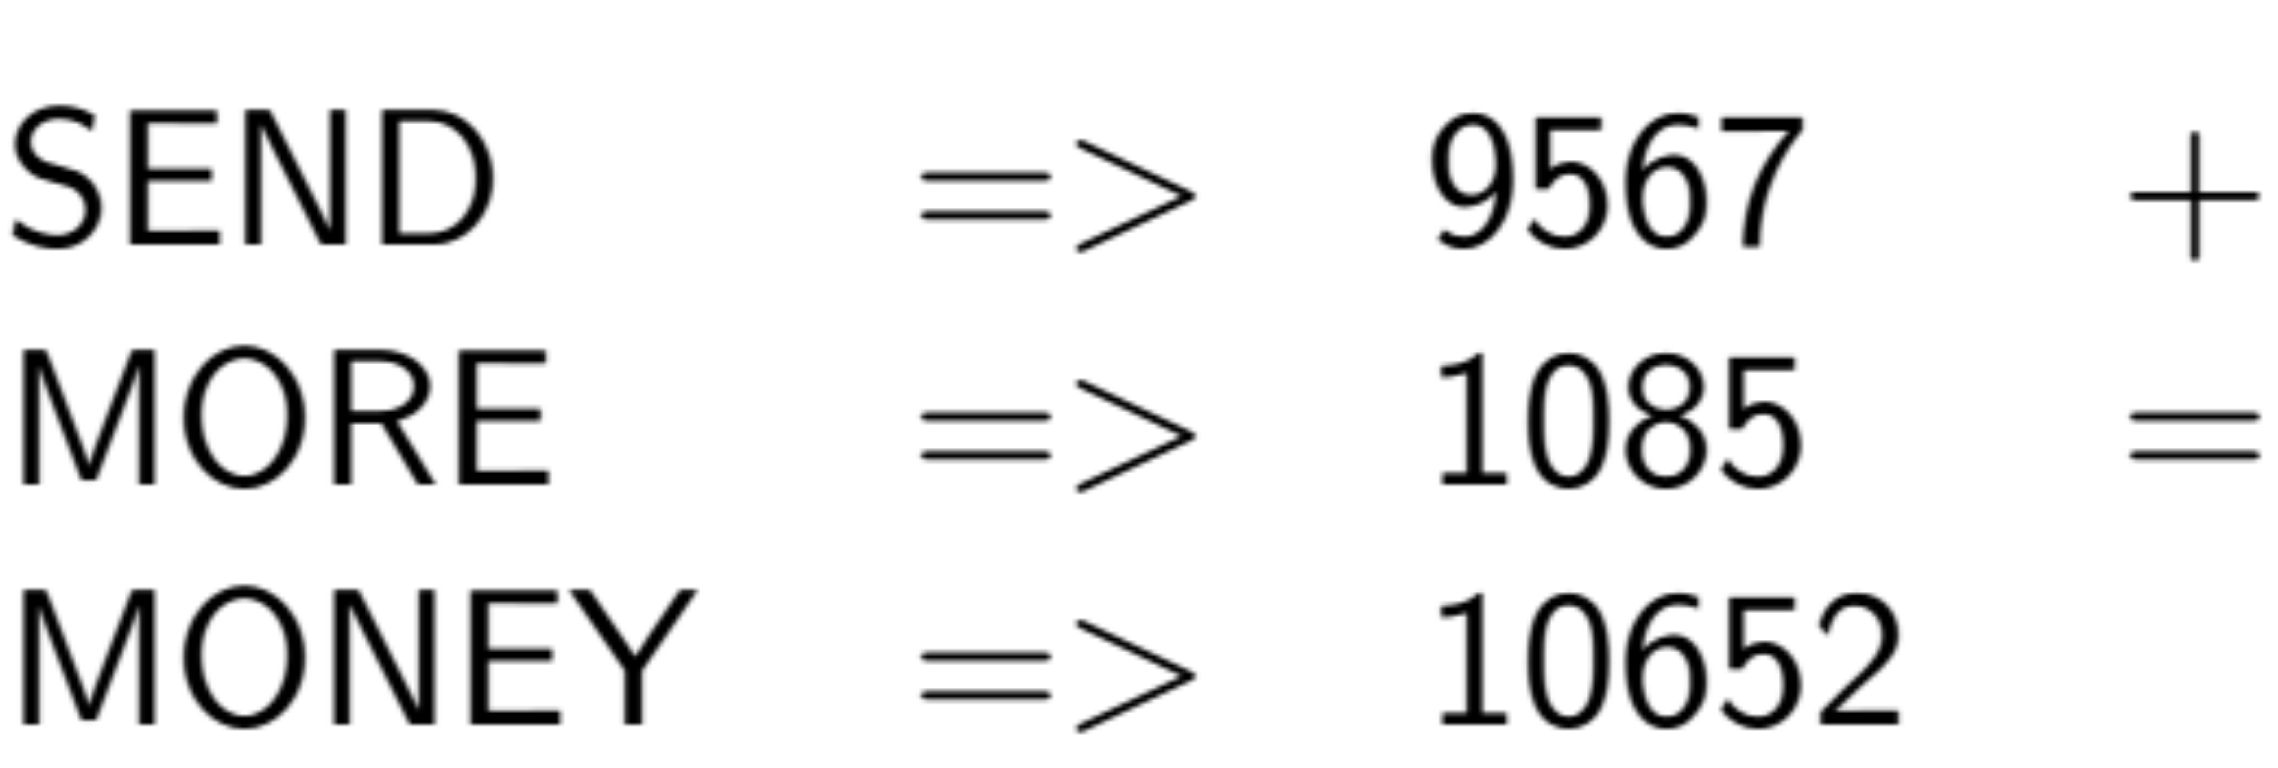
\includegraphics[scale=0.04]{img/money_result.png}
	\end{columns}

\end{frame}

\section{JSetL}
\begin{frame}{What is JSetL?}
	\begin{columns}
		\column{0.75\textwidth}
        	\begin{itemize}
        	\setlength\itemsep{2em}
			\item \textbf{JSetL} is a Java library that has been developed at the University of Parma since 2002.\\
			(\url{http://www.clpset.unipr.it/jsetl/})\\
			\item It allows the user to use a \textbf{declarative programming style} inside Java, making it very easy to \textbf{declare and solve constraints} on logical objects.
			\end{itemize}

		\column{0.25\textwidth}
			
\includegraphics[scale=0.3]{img/JSetL.png}
	\end{columns}
\end{frame}

\begin{frame}{Main Features}

JSetL combines the classical O-O paradigm of Java with some \textbf{typical concepts} of the \textbf{constraint logic paradigm}, such as:
\vspace{5 mm}
\begin{itemize}
\setlength\itemsep{2em}
        	\item Logical variables
        	\item Unification
        	\item Constraints resolution
        	\item Non-determinism
	\end{itemize}      
\end{frame}

\begin{frame}{JSetL classes}

JSetL offers a series of useful \textbf{Java classes}, in order to fully support the declarative style we discussed.\\
Some of these classes are:
\vspace{5mm}
\begin{itemize}
\setlength\itemsep{2em}
\item LVar
\item LSet
\item Constraint
\item Solver
\end{itemize}

\end{frame}



\begin{frame}[fragile]
\frametitle{LVar}
\begin{itemize}
\setlength\itemsep{3em}
\item The class \texttt{LVar} implements the concept of \textbf{logical variable}, as already seen in Prolog: a variable in a logic programming language is initially undefined (\textbf{unbound}), but may get \textbf{bound} to a value or another logic variable during unification of the containing clause with the current goal.\\
The value bounded to the variable may contain other variables which may themselves be bound or unbound.\\
\item Clearly, this is \textbf{quite different} from the concept of variable in the \textbf{imperative paradigm}!\\

\end{itemize}
\end{frame}

\begin{frame}[fragile]
\frametitle{LVar}
Examples:\\

\begin{lstlisting}
/* Creation of an unbounded LVar (no associated name) */
LVar A = new LVar();

/* Creation of a LVar bounded to the integer 1 (no associated name) */
LVar B = new LVar(1);

/* Creation of a LVar bounded to the integer 3, with associated name "C" */
LVar C = new LVar("C", 3);
\end{lstlisting}

A special subclass of \texttt{LVar} is \texttt{IntLVar}:
\begin{lstlisting}
/* Creation of an unbounded IntLVar which can assume integer values in [0..9], with associated name "X" */
IntLVar D = new IntLVar("X", 0, 9);
\end{lstlisting}
These kind of \texttt{LVar} objects are very important, because we can apply to them constraints like \texttt{sum}, \texttt{mul}, and many others.
\end{frame}


\begin{frame}[fragile]
\frametitle{LSet}
\begin{itemize}
\setlength\itemsep{2em}
\item The class \texttt{LSet} implements the concept of a \textbf{logical object collection}, organized in the form of a \textbf{mathematical set}.\\
\item A logical set can contain any other object (in particular, other \texttt{LSet} objects), ignoring any element repetition.\\
\item Similarly to \texttt{LVar}, \texttt{LSet} object can be bound or unbound, but they can also be \textbf{completely} or \textbf{partially specified}!\\

\end{itemize}

\end{frame}

\begin{frame}[fragile]
\frametitle{LSet}
Examples:\\

\begin{lstlisting}[mathescape]
/* Creation of an unbounded LSet without any associated name
   (it represent a completely variable(unspecified) set) */
LSet A = new LSet();

/* Creation of a completely specified set, bounded and without any associated name
   (it represents the set {1,2,3}) */
LSet B = LSet.empty().ins(1).ins(2).ins(3);

/* Creation of a partially specified set, unbounded and with associated name "C"
   (it represents the set {_LV1, _LV2} $\color{gray} \cup$ C)
   (note that the first two LVar have no associated name) */
LSet C = new LSet("C").ins(new LVar()).ins(new LVar());
\end{lstlisting}

\end{frame}




\begin{frame}[fragile]
\frametitle{Constraint}
\begin{itemize}
\setlength\itemsep{2em}
\item The class \texttt{Constraint} implements the concept of \textbf{logical constraint} in JSetL.\\
\item A constraint is a \emph{relation} that can be applied to a logical variable (\texttt{LVar}) or to a logical set (\texttt{LSet}).\\
\item It can be either \emph{atomic} or \emph{composed}.\\
\end{itemize}
\end{frame}

\begin{frame}[fragile]
\frametitle{Constraint}
\begin{itemize}
\setlength\itemsep{2em}
\item \textbf{Atomic constraints}, which can be:\\
\begin{itemize}
\item The \emph{empty} constraint (denoted as \texttt{[]})\\
\item $ e_{0}.op(e_{1},...,e_{n}) $ or $op(e_{0},e_{1},...,e_{n}) $ with $ n = 0,...,3 $\\
where $op$ is the constraint name, and $e_{i} (0 \le i \le 3)$ are expressions whose type depends on $op$.\\
\end{itemize}
\item \textbf{Composed constraints}, which can be obtained by:
\begin{itemize}
\item Conjuction ($ c_{1}.and(c_{2}) $)
\item Disjunction ($ c_{1}.or(c_{2}) $)
\item Implication ($ c_{1}.impliesTest(c_{2}) $)\\
\end{itemize}
\end{itemize}
\end{frame}

\begin{frame}{Some constraints on LSet}
\begin{table}[]
\begin{tabular}{|l|l|l|}
\hline
\textsc{Constraint}     & \textsc{JSetL}           & \textsc{Semantic}\\ \hline
Equality  	 & \texttt{A.eq(B)}                 & \texttt{A} $=$ \texttt{B}                        \\ \hline
Disjunction  & \texttt{A.disj(B)}           & \texttt{A} $\cap$ \texttt{B} $=$ $\varnothing$   \\ \hline
Union        & \texttt{A.union(B,C)}    & \texttt{C} $=$ \texttt{A} $\cup$ \texttt{B}      \\ \hline
Intersection & \texttt{A.inters(B,C)}  & \texttt{C} $=$ \texttt{A} $\cap$ \texttt{B}      \\ \hline
Difference   & \texttt{A.diff(B,C)}      & \texttt{C} $=$ \texttt{A} $\setminus$ \texttt{B} \\ \hline
\end{tabular}
\end{table}
\end{frame}


\begin{frame}[fragile]
\frametitle{Solver}
\begin{itemize}
\setlength\itemsep{2em}
\item The \textbf{constraint solver} is implemented by the class \texttt{Solver}.\\
\item This class provides methods to \textbf{add, show} and \textbf{solve} constraints.\\
\item Constraints are solved through \textbf{syntax-rewriting rules}, and the solving algorithm ends when there are no more rules to apply (or when a \texttt{Failure} exception is thrown, in the case of a non satisfiable constraint).\\
\end{itemize}
\end{frame}

\begin{frame}[fragile]
\frametitle{Solver class methods}
These are the main methods provided by the \texttt{Solver} class:\\
\begin{itemize}
\item public void \textbf{add}(Constraint c)\\ 
Adds the constraint \texttt{c} to the constraint store of the solver.\\
\item public void \textbf{showStore}()\\ 
Prints the conjuction of all the constraint in the constraint store which are still in a non-solved form.\\
\item public void \textbf{solve}()\\ 
Tries to solve the constraints in the constraint store: if they are not satisfiable, it throws a \texttt{Failure} exception.\\
\item public boolean \textbf{check}()\\ 
Like \texttt{solve()}, but no exceptions are thrown: it just returns \texttt{true} if the constraints in the constraint store are satisfiable, \texttt{false} otherwise.\\
\end{itemize}

\end{frame}

\begin{frame}[fragile]
\frametitle{SEND + MORE = MONEY with JSetL}
Let's try to implement the previous SEND + MORE = MONEY puzzle seen before in Prolog, this time in Java using JSetL:\\
\begin{exampleblock}{Money.java}
\begin{lstlisting}
		IntLVar s = new IntLVar("S", 0, 9);
		/*...*/
		IntLVar money = new IntLVar("MONEY");
		IntLVar[] letters = {s, e, n, d, m, o, r, y};
		Solver solver = new Solver();
		
		/* S >= 1 and M >= 1 */
		solver.add(s.ge(1).and(m.ge(1)));

		/* Each variable is different from each other */
		solver.add(Constraint.allDifferent(
			(Object[]) letters)
		);
\end{lstlisting}
\end{exampleblock}
\end{frame}

\begin{frame}[fragile]
\frametitle{SEND + MORE = MONEY with JSetL}
\begin{lstlisting}
		/* SEND = S*1000 + E*100 + N*10 + D */
		solver.add(send.eq(s.mul(1000).sum(e.mul(100).sum(n.mul(10).sum(d)))));
		
		/* MORE = M*1000 + O*100 + R*10 + E */
		solver.add(more.eq(m.mul(1000).sum(o.mul(100).sum(r.mul(10).sum(e)))));
		
		/* MONEY = M*10000 + O*1000 + N*100 + E*10 + Y */
		solver.add(money.eq(m.mul(10000).sum(o.mul(1000).sum(n.mul(100).sum(e.mul(10).sum(y))))));
		
		/* MONEY = SEND + MORE */
		solver.add(money.eq(send.sum(more)));
		
		/* Labeling on the variables */
		solver.add(s.label());
		/*...*/
		
		/* Try to find a solution */
		solver.solve();
	
\end{lstlisting}
\end{frame}

\begin{frame}{  }
\centering \huge Thanks for your attention!
\end{frame}

\end{document}
